% credit: https://github.com/makokal/beamer-themes
\documentclass{beamer}
\usetheme{ALUF}

\usepackage[utf8]{inputenc}
% \usepackage{palatino}
% \usepackage[T1]{fontenc}
\usepackage{lmodern}
\usepackage[expert]{mathdesign}
\usepackage[protrusion=true,expansion=true,tracking=true,kerning=true]{microtype}

\usepackage{algorithm2e}
% \usepackage{multimedia}
\usepackage{media9}
\usepackage{multirow}

\title{Facial emotion recognition with latent topics modeling on local features}
\subtitle{AI project}
\author{Vo Thanh Hung}
\date{June 2019}
% \institute{\url{email@some-cool-place.ext}\\\url{http://www.cool-url.com}}

\graphicspath{ {imgs/} }
\begin{document}

\begin{frame}[plain,t]
\titlepage
\end{frame}

\begin{frame}% [plain,t]
	\frametitle{Outline}
\tableofcontents
\end{frame}

%=============================================================================================

% -----------------------------------
% FER introduction
% -----------------------------------
\section{Introduction}
\begin{frame}{Facial emotion recognition (FER)}
\begin{figure} [h!]
\centering
\begin{tabular}{|c|c|c|c|c|c|c|}
  \hline
  \tiny Surprise & \tiny Fear & \tiny Disgust & \tiny Happiness & \tiny Sadness & \tiny Anger & \tiny Neutral \\
  \addheight{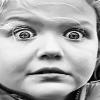
\includegraphics[width=.1\textwidth]{imgs/train_00006_aligned-1.jpg}} &
  \addheight{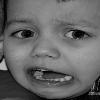
\includegraphics[width=.1\textwidth]{imgs/train_00027_aligned-2.jpg}} &
  \addheight{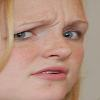
\includegraphics[width=.1\textwidth]{imgs/train_00031_aligned-3.jpg}} &
  \addheight{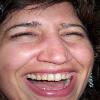
\includegraphics[width=.1\textwidth]{imgs/train_00016_aligned-4.jpg}} &
  \addheight{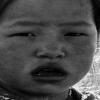
\includegraphics[width=.1\textwidth]{imgs/train_00005_aligned-5.jpg}} &
  \addheight{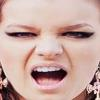
\includegraphics[width=.1\textwidth]{imgs/train_00047_aligned-6.jpg}} &
  \addheight{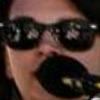
\includegraphics[width=.1\textwidth]{imgs/train_09757_aligned-7.jpg}} \\

  \addheight{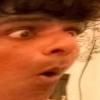
\includegraphics[width=.1\textwidth]{imgs/test_0043_aligned-1-2.jpg}} &
  \addheight{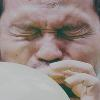
\includegraphics[width=.1\textwidth]{imgs/test_0274_aligned-2-2.jpg}} &
  \addheight{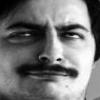
\includegraphics[width=.1\textwidth]{imgs/train_09745_aligned-3-2.jpg}} &
  \addheight{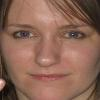
\includegraphics[width=.1\textwidth]{imgs/test_0055_aligned-4-2.jpg}} &
  \addheight{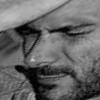
\includegraphics[width=.1\textwidth]{imgs/test_0049_aligned-5-2.jpg}} &
  \addheight{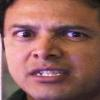
\includegraphics[width=.1\textwidth]{imgs/test_0057_aligned-6-2.jpg}} &
  \addheight{
\includegraphics[width=.1\textwidth]{imgs/train_09759_aligned-7-2.jpg}} \\
  \hline
\end{tabular}
\caption{Example images from RAF-DB}
\label{fig:raf-db-example}
\end{figure}
\end{frame}

\begin{frame}{next}
    
\end{frame}

\section{Related work}
\begin{frame}{Image feature extraction}
    \begin{itemize}
        \item<1-> SIFT
        \item<2-> SUFT
        \item<3-> KAZE
        \item<4-> etc.
    \end{itemize}
\end{frame}

\begin{frame}{Bag-of-Words}
    
\end{frame}

\begin{frame}{Latent topics modeling}
    \begin{itemize}
        \item<1-> LDA
        \item<2-> HDP
    \end{itemize}
\end{frame}

\section{System architect}
\begin{frame}{System architect}
    \begin{figure}
        \centering
        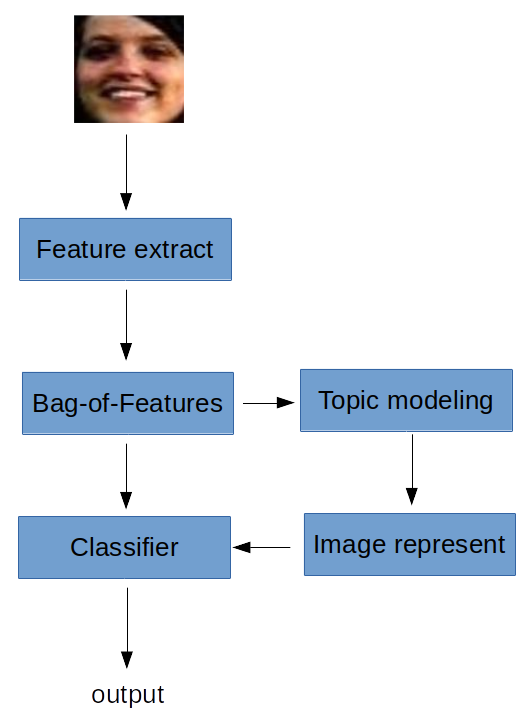
\includegraphics[width=.45\textwidth]{system-arch-cropped.png}
        \caption{System architect}
        \label{fig:system-architect}
    \end{figure}
\end{frame}

\section{Experiments and results}
\begin{frame}{Dataset}
    RAF-DB
\end{frame}

\begin{frame}{Configure + ...}
    
\end{frame}

\begin{frame}{Results}
    
\end{frame}

% ---------------------------------
% SUMMARY
% ---------------------------------
% \section{Summary}
\begin{frame}{}
  \centering \Large
  \emph{Thank you!}
\end{frame}

%\ThankYouFrame

\end{document}
